\chapter{Subspaces}
Shark philosophy is straightforward. Peers collect data in their
knowledge bases. They can create interests and expose it to other 
peers. A communication takes place of a mutual interest is identified.

That's quite similar to the well-know WWW concept: A client asks a 
server for a document and gets a reply.

Apparently, that's not sufficient for a number of Web 2.0 applications.
A chat, a forum, project sites etc. are means to exchange documents 
between people who share similar interests e.g. participate in the same
project.

Server-based applications create a database on a dedicated machine
and offer restricted access to that machine. Figure X illustrates that
-- well known -- concept.

That concept of sharing documents in a (open or closed) group 
of users can also be created in the realm of P2P networks. 
{\it Sub spaces} are the Shark concept for that purpose.

\section{Concept}
Each subspace contains a knowledge base. It can contain -- as each knowledge base -- context points with properties and information. Subspaces are created by a peer which automatically becomes {\it owner} of that subspace. 

Each subspace is unique. It requires a unique subject identifier. The framework offers methods to create those unique identifiers. Subspace owner can {\it invite} other peers. Invited peer get an invitation. They can decide whether to join the subspace or not. They simply ignore the invitation in the later case.

Invited peers can {\it subscribe} to a subspace. A local knowledge base is created with the same subject identifier as the original subspace created by
the owner. 

Peers can add context points and information to subspaces. Each invited peer -- and the owner is per definition invited -- gets a copy of those new context points or information. Subspaces are actually just means to synchronize copies of its containing knowledge base.

Peers can unsubscribe from subspaces. They won't get new information any longer. They local copy still remains until it is finally removed by the peer. Owner can remove peers from subspace. It has the same effect as if a peer 
would unsubscribe.

The subscription types can be distinguished: {\it full member} and {\it read-only member}. The meaning obvious: Full member can add data to their subspaces. An attempt by a read-only member would fail. 

Data can be removed from subspaces. {\bf Note, removing data is not propagated to other subspaces}. It is up to applications to propagate data removal\footnote{That rule sounds odd in first place. It has an advantage though. Imagine a chat. A peer might decide to remove a number of chat entries. What should a subspace do? Removing the copies in all subscribed knowledge bases wouldn't be an expected behaviour. Imagine, Alice, Bob and Clara an in a chat. Bob decides to remove any discussion between Alice and Clara. What would Alice and Clara think if their local copies would be lost as well. Therefore, subspaces propagate new data but not data removal.}.

Each peer is free to unsubscribe from a subspace at any time. Owner can not. They can {\it destroy} the subspace which means that any subscriber is unsubscribed. Local copies remain intact. Such destroyed subspaces are actually
archives which cannot be changed. Each peer is free to remove it, though.

There are two kind of subspaces: {\it Closed} and {\it open} subspaces. Closed subspaces has been described until now. They have an owner which can invite and unsubscribe peers. Open subspaces are slightly different. There are created as well by a peer. Each peer can subscribe to such subspaces without interaction with the owner peer. Open subspace owner have no specific privileges except the fact that they have created the subspace. The cannot unsubscribe peers. Each peer can subscribe if it pleases.

Peers can create a subspace clone. A new subspace with a different identity (which means different subject identifier) is created. Clones knowledge base is empty. What is cloned than? The subscriber list. The cloning peer becomes owner of the cloned subspace. Each member of the cloned subspace is invited to the new clone. 

This feature was introduced to underline the decentralized character of Shark. Closed subspaces introduced a hierarchy. That's useful in many cases. Nevertheless, a peer shouldn't have to much power over others in such a libertarian system even in a subspace. Each peer can decide to leave a subspace and it can also to decide other peers to follow. Such effects can be seen from time to time in social networks. A forum becomes somewhat weired. Fractions of users start to fight each other. Cloning is a solution. A peer of one fraction creates a clone, removes any peer from the opposite fraction and invites all of its friends. Now, they have their own subspace.

The next sections explain subspace usage on the API level.

\section{Implementation details}
Creating a subspace is somewhat tricky. Subspaces are a powerful tool and
provides a lot of feature that are required to produce community in a P2P 
environment. The next pages might be a bit complicated. It is worth studying it, though.

Subspace functionality is mostly implemented in {\tt InMemoSubSpace} in the 
{\tt net.sharkfw.subspace} package. As the name implies, this class doesn't offers any persistency. Derived class {\tt net.sharkfw.subspace.filesystem.FSSubSpace} does. Other persistent implementations will follow.

We have to present two other entities before discussing details. 
There is another class {\tt SubSpaceGuardKP}. Shark engines working with subspace must run a single object of this class\footnote{Actually, more than
one guard KP can be instantiated. We don't discuss this kind of subspace multiversum in this version of the programmers guide. Maybe later. Up to here, take it as a rule: Use the guard KP as singleton. It's better and has actually no serious drawbacks.}.

Subspaces communicate with KEP. They use a special coding which prevents other knowledge ports from processing those messages, see \ref{subspacemessages}.
For example, when a peer inserted new data into its local subspace, a message is
send to each subscribed peers in order to notify about this event. Subspace owner can
invite another peer. Both subspace specific messages are encapsulated into KEP messages. The guard KP takes any subspace message and performs necessary actions. Here is the good news for any developer: You have nothing to do with the communication. The whole synchronization process is already in place. You have just to handle several events which can arise. And you have to create the guard object.

The guard requires a shark engine, a shark knowledge base and an object that implements {\tt SubSpaceManager}. The engine is pretty clear. It's the engine that makes up the shark peer. The knowledge base shall is called the {\it baseKB}. What makes that kb special. Actually nothing in the first place, but it becomes interesting: We have already learned that peers can be invited and can subscribe. Those, peers can learn about other peers or try to invite peers. The peer descriptions, namely the peer semantic tags must be stored somewhere. The peer dimension of the baseKB is that place. 

Before setting up subspaces, find a knowledge base the will hold all new peers.
Most shark peers will work with a single knowledge base. That's wise and makes the decision easy. Take the only knowledge base as baseKB and be aware of a growing peer dimension.

{\tt SubSpaceManager} is an interface providing three methods:

\begin{verbatim}
public Iterator<SubSpace> getSubSpaces() throws SharkKBException;
public SubSpace getSubSpace(String si) throws SharkKBException;

public void invitedToSubSpace(String subSpaceName, 
    String subSpaceSI, 
    String subSpaceType, 
    SemanticTag subSpaceTopic,
    String parentSpaceSI, 
    String childString,
    PeerSemanticTag remoteOriginator, 
    ArrayList<PeerSemanticTag> member, 
    ArrayList<PeerSemanticTag> roMember, 
    boolean subSpaceOpen, 
    boolean readonlyInvitation) 
    throws SharkSubSpaceException, 
        SharkNetException, 
        SharkKBException, 
        SharkSecurityException;
\end{verbatim}

First method is expected to return an iteration of known subspaces in this shark peer. The seconds methods shall return a subspace with a give subject identifier. Apparently, it is assumed that the subspace manager shall be aware of all existing subspaces. Shark offers a simple implementation of such a subspace manager, see class {\tt SimpleSubSpaceManager}.

The third methods is a called by the guard if a new invitation has arrived and a corresponding subspace does not yet exist on this peer. In most cases, the subspace manager will ask the user whether to join or not and will create a local copy of the subspace.

Following figure gives an overview on the objects that make up the subspace environment.

%\begin{figure}[t]
%\centering
%\includegraphics[width=0.40\textwidth]{subspaceEnvironment.eps}
%\caption{All objects making up the subspace environment}
%\label{fig:subspaceEnvironment}
%\end{figure}

\subsection{Creating a subspace}

\subsection{Creation process in detail}
This subsection can be skipped if an existing implementation is sufficient for application needs. It gives a bit more insights in the creation process.

{\tt ImMemoSubSpace} offers a single constructor which takes just a single parameter a {\tt SubSpaceGuardKP}

\subsection{Subspace messages}
\label{subspacemessages}
This section can be skipped...


\section{Basic structures}
\begin{figure}[t]
\centering
\includegraphics[width=0.40\textwidth]{subspace.eps}
\caption{Sub space stores its data in its own knowledge base.}
\label{fig:subspace}
\end{figure}

Let's start with basic data structures and discuss communication principles later. A sub space is stored in a peer. A subspace comprises its own knowledge base and two additional peer lists: {\it member} and {\it read only member}.
A subspace is created by a peer which became {\it owner}.

Figure \ref{fig:subspace} illustrates these relationship. Peer {\it Alice} has apparently created a new subspace. She defined Bob and Clara as member of that sub space whereas Bob is a {\it full member} and Clara just {\it read only member}.

Creating a subspace is straightforward.
\begin{verbatim}
Add sample code here.
\end{verbatim}

Member can be invited into a subspace after its creation.

There are two methods: {\verb|inviteAll()|} can only be called once. It is meant to be used directly after subspace creation to introduce all member to the newly created subspace. Subsequent calls of {\verb|inviteAll()|} has no effect after its first successful execution.

\begin{verbatim}
SubSpace aliceSubSpace =..;
aliceSubSpace.inviteAll();

if(aliceSubSpace.allInvited()) {
    // worked perfectly
    System.out.println("Invitation has been sent");
}
\end{verbatim}

Member can be added after creation by means of {\verb|addFullMember()|} or
{\verb|addReadonlyMember()|} Both methods have a single parameter namely a \newline
{\verb|PeerSemanticTag|} which is to be invited into the subspace.

{\it Note, only subspace owner can invite new member.}

Member can be removed with {\verb|removeMember()|}. This method can also only be called by the owner.

Each subspace member can get a list of all subspace member by using 
{\verb|member()|}. Results differ slightly. Subspace owner get actually any member
of the subspace - regardless if peer has already subscribed to subspace or not.

Each member that is not owner only gets a list of {\it subscribed} member.

\subsection{Entering and leaving subspaces}
Subspace member are invited by subspace owner. A system that accepts subspace invitations must run a {\verb|SubspaceGuardKP|}. That special Knowledge Port is 
created like this:

\begin{verbatim}
SubSpaceManager sne =..;
SharkKB kb=..;

KnowledgePort guardKP = new SubspaceGuardKP();
\end{verbatim}

The following section describes some details of the guard KP. You can ignore that section if you are not interested in details of sub space communication.

\subsubsection{SubSpaceGuardKP}


\subsubsection{Subscribing}
Non-owner are invited to subspaces. A {\verb|SubSpaceGuardKP|} creates an empty subspace after receiving an invitation\footnote{Note, this behaviour can be overwritten. Sometimes, it might not be useful to created subspaces without
further user interactions - see previous section for details.}.

\begin{figure}[t]
\centering
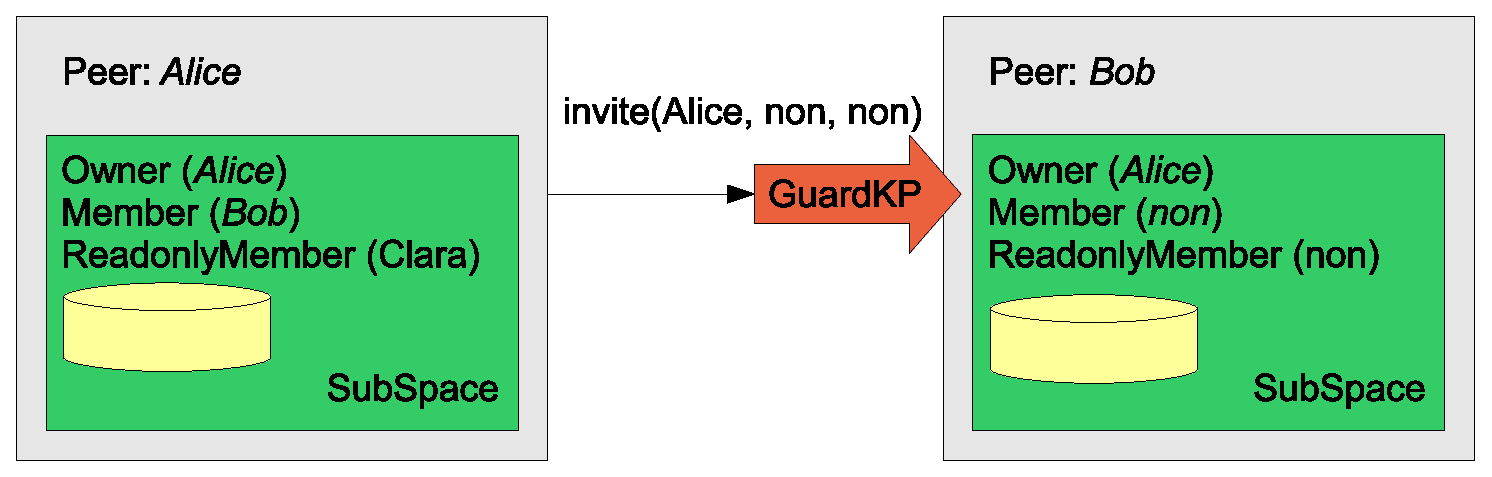
\includegraphics[width=0.60\textwidth]{subspaceAfterInvitation.eps}
\caption{Peers invited but not subscribed}
\label{fig:subspaceAfterInvitation}
\end{figure}

Figure \ref{fig:subspaceAfterInvitation} illustrates that situation.
Alice has invited Bob (beside Clara which isn't shown in th figure). The 
SubSpaceGuardKP has created the sub space in the Bob peer. Have a look
at the member lists. Only {\it Alice} as owner is known subspace because member.

Bob has two options: He can subscribe to the subspace or not. He hasn't to inform Alice if he doesn't want to enter the subspace. He can just remove the subspace from its system and is done.

Subscribing is pretty easy:

\begin{verbatim}
SubSpace aliceSubSpace = ...;
aliceSubSpace.subscribe();
\end{verbatim}

Actually two things happen: Alice gets informed that Bob has joined the subspace. Furthermore, a {\verb|SubSpaceKP|} is created that handles communication with other (subscribed) peers of the subspace.

Figure \ref{fig:subSpaceRefreshing} illustrates action which are and can
be performed afterwards. Alice has already received Bobs' subscription message. 
Thus, subspace status has changed: Bob became subscribed member. Alice refreshes
Claras list of members. Clara subscribes as well in our example. That message
is performed by Alice as well and leads to a refreshing message to Bob.

\begin{figure}[t]
\centering
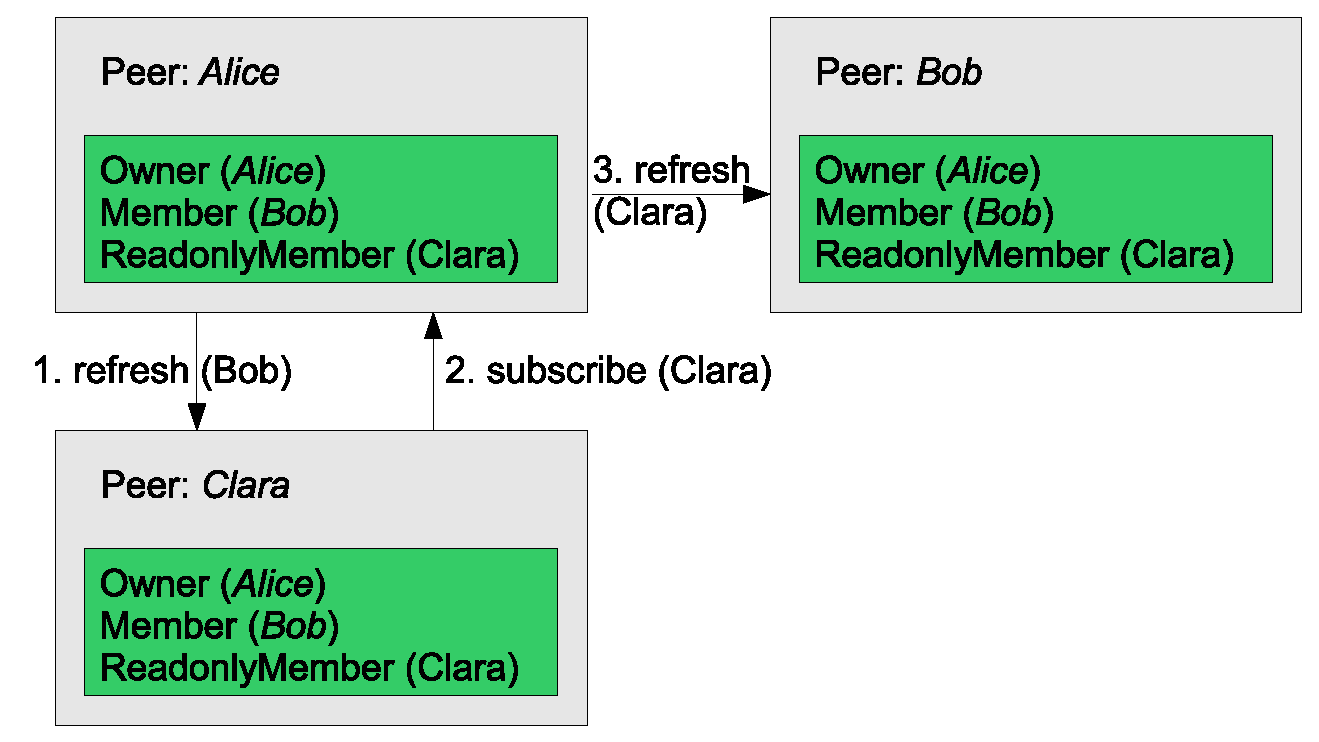
\includegraphics[width=0.60\textwidth]{subSpaceRefreshing.eps}
\caption{Refreshing subscription lists}
\label{fig:subSpaceRefreshing}
\end{figure}

Finally, any member has got the current subscription list.

The same procedure is performed when peers unsubscribe. An unsubscribe method changes member list in the owner which are propagated to all subspace members.

\subsection{Information exchange}
Member can add information to a subspace at any time. The data model doesn't differ from what we have already discussed until now. Peers can create context points and add information.

Subspaces differ in two ways: 

\begin{itemize}
\item 
Each locally added context point is sent
to each subscribed member.
\item 
Read only member are not allowed to add information into subspace knowledge
base. And attempt is answered with an exception.
\end{itemize}

Context point can be created with the subspace by using {\verb|createCP()|}. 
Information can be added now. The subspace automatically transmits any 
information that is added to all other subscribed peers.

Figure \ref{fig:subspaceAddingCP} illustrates this behaviour. The real user Alice adds information to her software. The Shark application uses a subspace for information storage and dissemination. Added information is stored locally in the Alice peer and also transmitted to any subscribed peer.

There is a callback method ({\verb|cpReached()|}) which is called when new
information has reached the subspace. Application can overwrite this method
what makes sense in most scenarios. Subspaces are e.g. used to implements 
chat rooms. A text or document is added in one peer and automatically 
distributed to others. The first peer is aware of new information due to
the performed user interaction. The other peer received those information
automatically via Shark. Their user interface needs to be informed to 
get refreshed. Use ({\verb|cpReached()|}) for such purposes.

This behaviour has implications:

\begin{itemize}
\item 
Only subscribed peer received added information. Thus, a peer doesn't get
automatically any information that was stored in the subspace. It only gets
information which are added after successful subscription.

\item 
Removing of information is not propagated. There are (yet) no means to inform
other peers about local deletion of information or whole context points.

\end{itemize}

\begin{figure}[t]
\centering
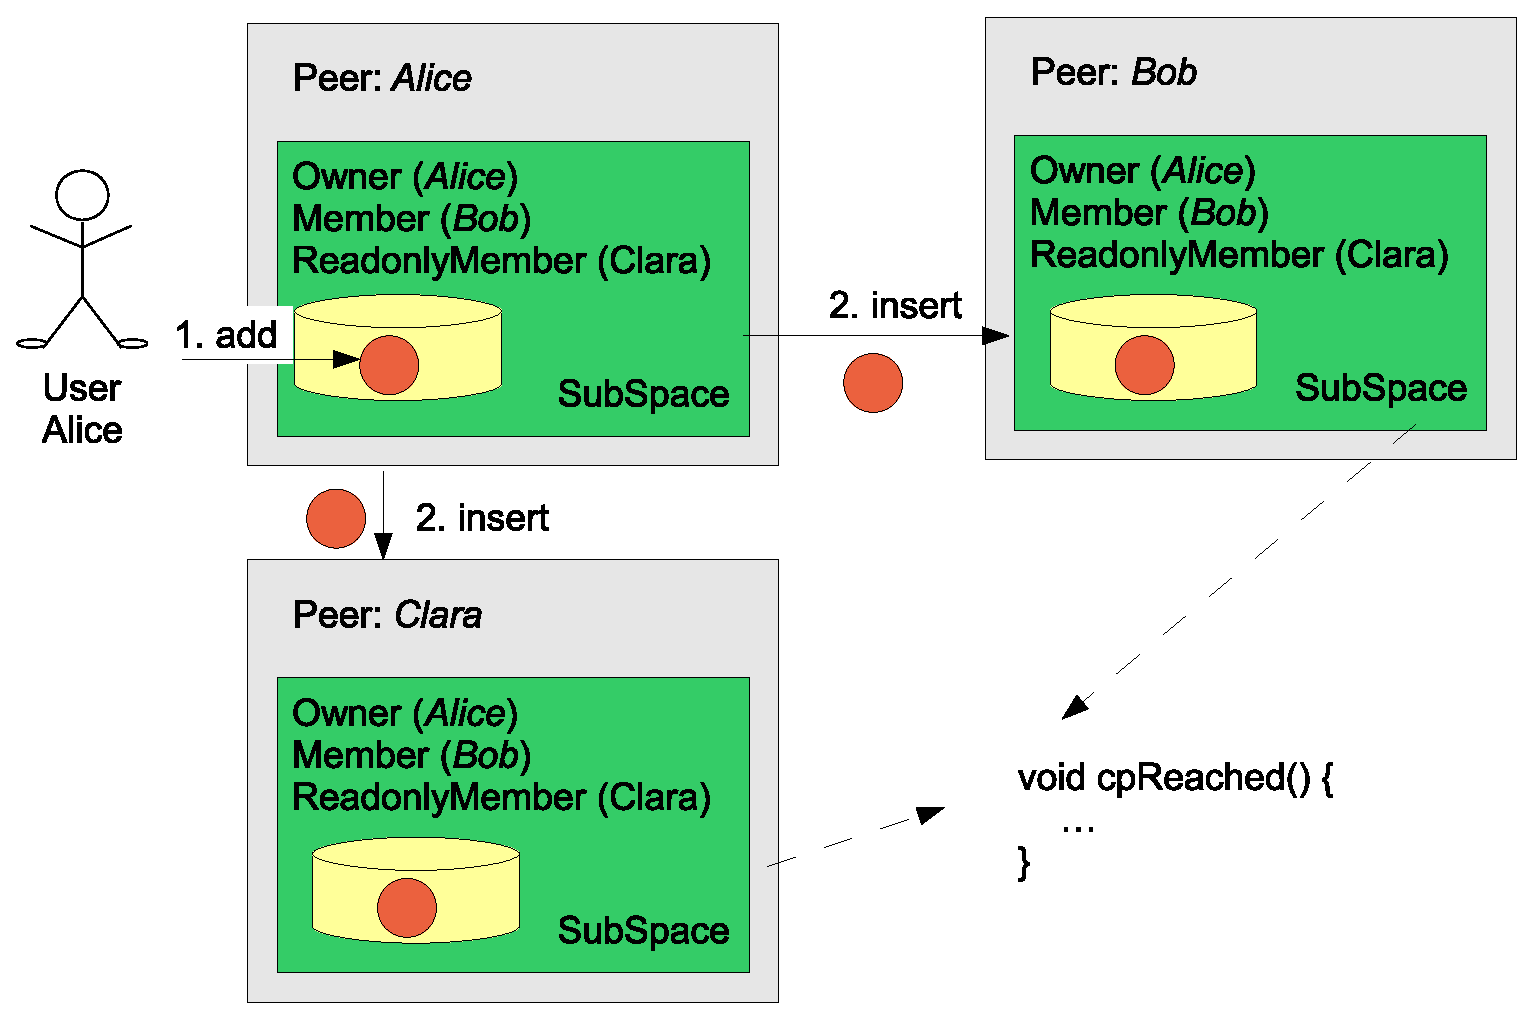
\includegraphics[width=0.60\textwidth]{subspaceAddingCP.eps}
\caption{Information synchronisation in sub spaces}
\label{fig:subspaceAddingCP}
\end{figure}

\subsection{Subspace knowledge base}

\section{Implementation details}
\subsection{Subspace Guard}
\subsection{Subspace KP}
\section{Implementing you own sub space}
\section{Using subspaces}

\section{Child sub spaces}

\section{Sub spaces usages}
\subsection{Chat}
\subsection{Makan}
\subsection{Forum}
\subsection{Shark Longitude}
